\documentclass{article}
\usepackage{graphicx} % Required for inserting images

\title{Test GithubSync}
\author{christoph.schult }
\date{\today}

\begin{document}

\maketitle

\section{Introduction}

\begin{itemize} 
    \item I am still trying to get started in Git and overleaf.
    \item But if you can read it, then I succeeded partly.
    \item This is because I made the changes on my work computer and pushed them to overleaf after that.
\end{itemize}

\section{Main part}
Just for fun, let's put a formula here: 
$$ (a + b)^2 = a^2 + b^2 + 2ab $$
This is the first binomial formula. 

I will add the second binomial rule, too:
$$ (a - b)^2 = a^2 + b^2 - 2ab $$

Surprise: There is even a third binomial formula!
$$ (a + b)(a - b) = a^2 - b^2 $$

\section{Why economics is great}
Economics provides us with many useful tools to understand the modern 
complex world and come up with solutions making the earth a better place.

Furthermore, economics is simply fun!

\section{Science is fun}
As \cite{holtem2024a} wrote, there is no significant effect on GVA in cities where Euro2024 took place. This finding challenged what was written more than a centrury ago by \cite{einstein1905}.

\section{Hello everyone!}
Just another useless paragraph to have some changes to add...

\begin{figure}
  \centering
  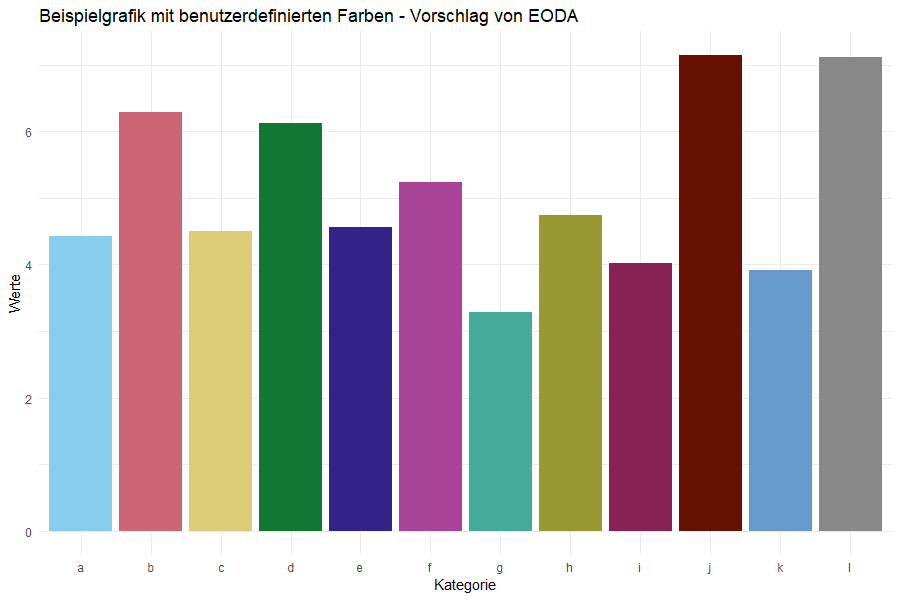
\includegraphics[width=\linewidth]{figures/EODA_cols_plot.png}
\end{figure} 

\subsection{Add a figure in overleaf}
Once more, a figure is added, this time in Overleaf. Let's see whether everything works as it should...

\begin{figure}
  \centering
  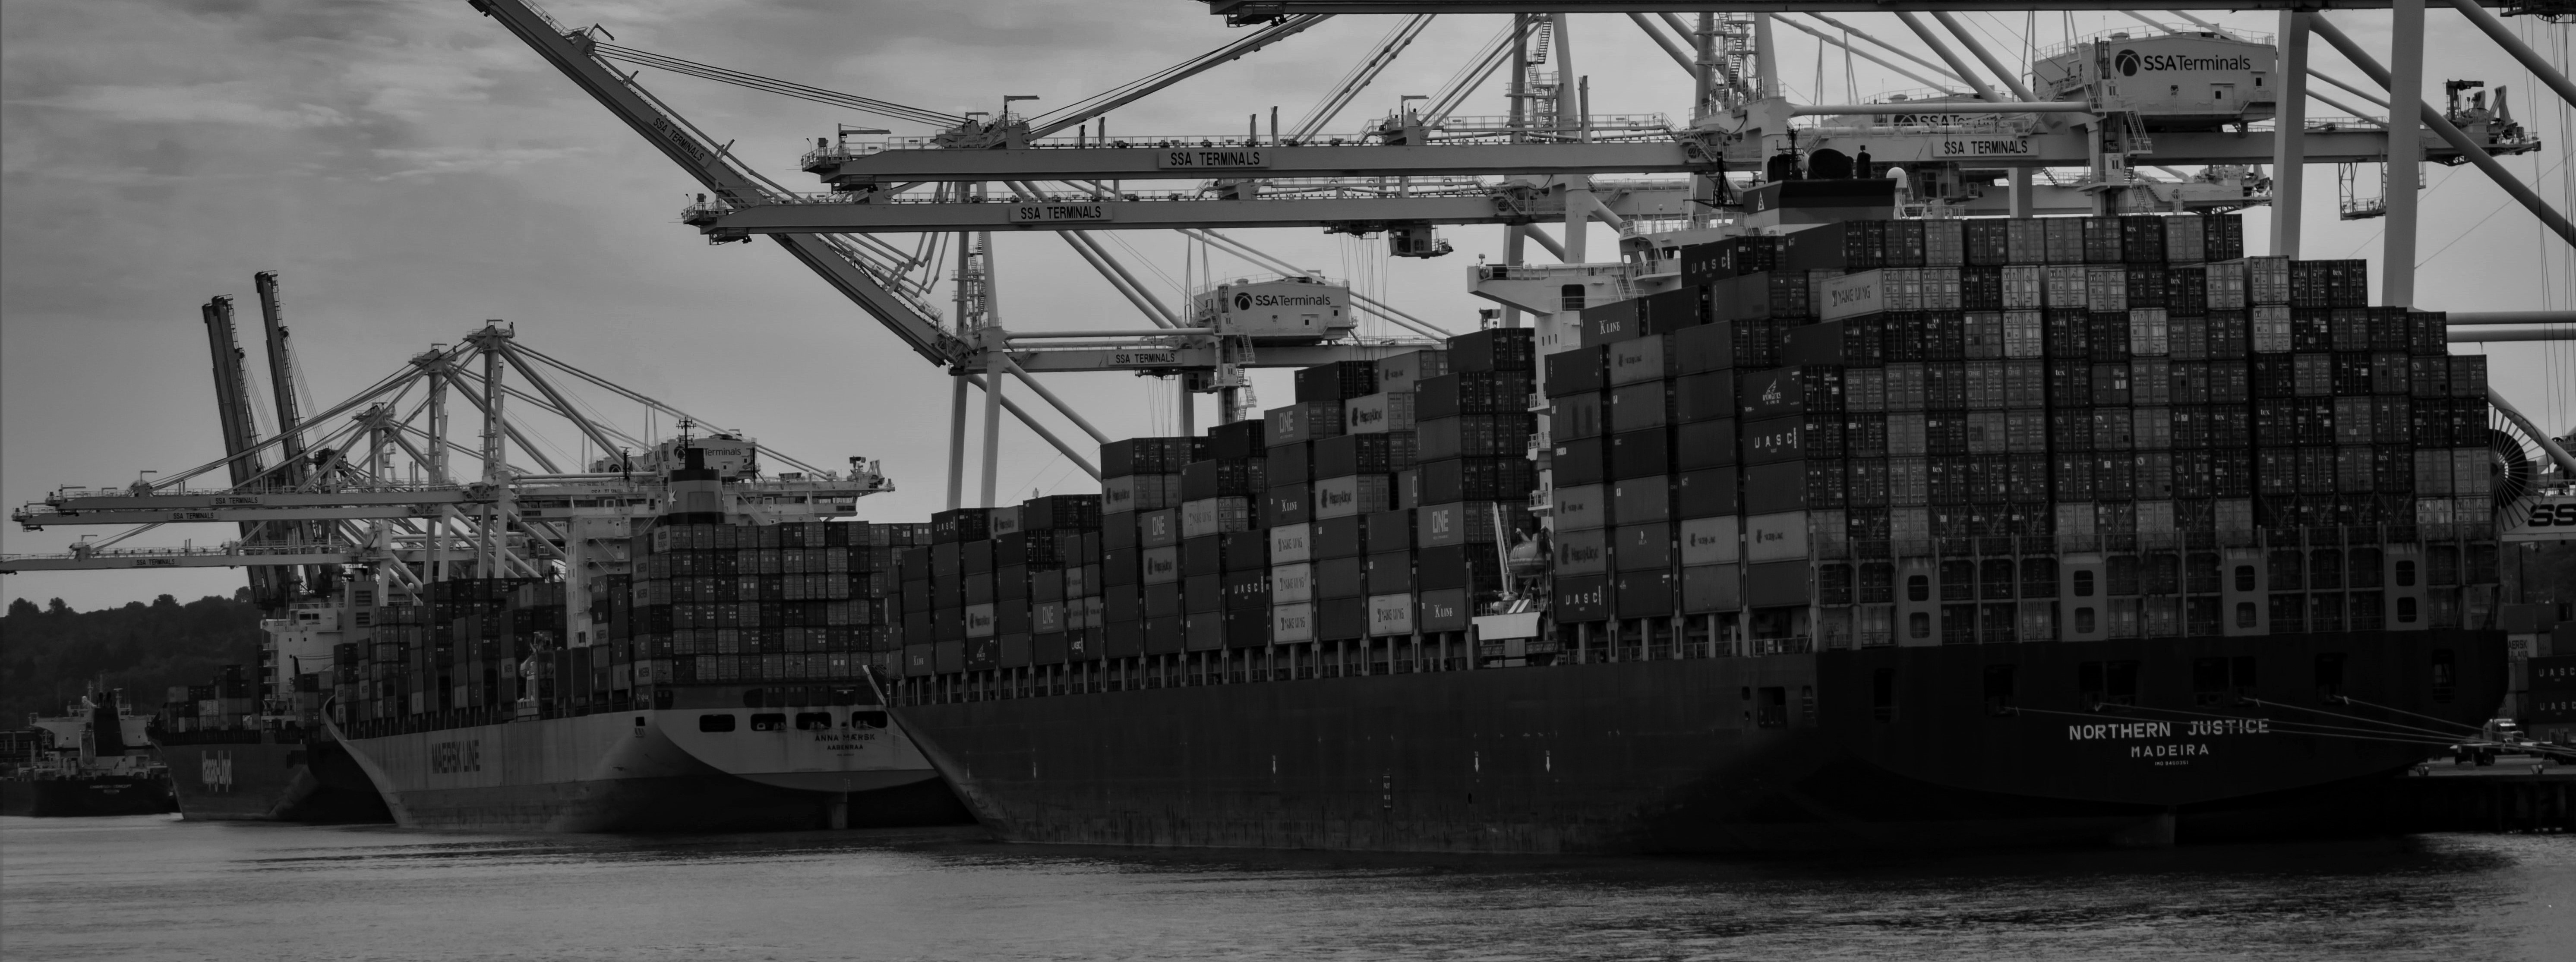
\includegraphics[width=\linewidth]{figures/Titelbild5grau_3.jpg}
\end{figure} 



\begin{thebibliography}{9}

\bibitem{holtem2024a} 
  A. Drygalla, K. Heinisch, O. Holtemöller (2024). 
  \textit{Gesamtwirtschaftliche Effekte von Fußball-Meisterschaften: Die WM 2006 und die EM 2024 in Deutschland}. 
  Konjunktur aktuell — Jg. 12 (2), 2024.


 \bibitem{einstein1905} 
 A. Einstein (1905). 
 \textit{Zur Elektrodynamik bewegter Körper}. 
 Annalen der Physik, 322(10), 891--921.

\end{thebibliography}


\end{document}
